\section{Техніко-економічне обґрунтування проекту}
\subsection{Обґрунтування доцільності розробки проекту}
На сучасному етапі розвитку складні логістичні системи вимушені працювати в умовах високої невизначеності, що суттєво ускладнює управління ними. 

В процесі прийняття управлінських рішень виникає проблема прогнозування поведінки системи та зовнішнього середовища. 
Результати прогнозів необхідно постійно коригувати по ходу розвитку подій, що дозволяє пристосовуватися до змін оточення та гнучко реагувати на негативні впливи. 

У нагоді тут стає агентне моделювання, яке сягає своїм історичним корінням складних адаптивних систем і принципу побудови систем знизу вгору.
Агентне моделювання дозволяє здійснити множину прогнозів за різними сценаріями залежно від формування різноманітних ситуацій практично необмеженої складності. 

Таким чином, дана інформаційна система є актуальною на сьогоднішній день, та дозволить швидко та практично досліджувати різні конфігурації розподільчої логістичної системи.

У даному розділі представлене техніко-економічне обґрунтування проекту по розробці ПЗ для аналізу функціонування розподільчих логістичних систем, а саме аналізу рівня ризиків та сервісу, рівня навантаження системи.

\subsection{Оцінка конкурентоспроможності у порівнянні з аналогом}
У якості програми для порівняння при розробці програмної компоненти був взятий інструмент FlexSim.
Цей продукт був обраний у якості аналогу на основі таких факторів: схожий профіль, відповідність вимогам технічного завдання проекту, доступність для дослідження аналогу у зв'язку з наявністю пробної версії.

Для оцінки конкурентоспроможності розроблюваного продукту необхідно провести аналіз і порівняння з обраним аналогом за функціональним призначенням, основним технічним та експлуатаційним параметрам, областям застосування. 
Подібний аналіз виконується за допомогою оцінки експлуатаційно-технічного рівня розроблюваного продукту.

Експлуатаційно-технічний рівень (ЕТР) розроблюваного продукту --- це узагальнена характеристика його експлуатаційних властивостей, можливостей, ступеню новизни, що є основою якості продукту. 
Для визначення ЕТР продукту можна використати індекс експлуатаційно-технічного рівня $J_\textup{ЕТР}$, який розраховується як сума часткових індексів, куди входять показники якості програмного продукту. 
Тоді
\begin{equation}\label{eq:economy_j_etp}
	J_\textup{ЕТР} = \sum^n_{j=1} B_j X_j,
\end{equation}
\begin{description}
	\item[де] $J_\textup{ЕТР}$ --- комплексний показник якості продукту;
	\item $B_j$ --- коефіцієнти вагомості $j$-го показника у частках одиниці, що призначається у відповідності до потреб організації-замовника програмного продукту;
	\item $X_j$ --- експертна оцінка $j$-го показника якості за вибраною шкалою оцінювання;
	\item $n$ --- число показників, що розглядається.
\end{description}

В таблиці~\ref{tab:economy_quality} представлені результати розрахунку бально-індексним методом за п'ятибальною шкалою оцінювання.

{
	\small
	\tabulinesep=1.2mm
	\begin{longtabu} to \textwidth {|X[3,l]|X[2,c]|X[1,c]|X[1,c]|X[1,c]|X[1,c]|}
  		\caption{Розрахунок показника якості}
  		\label{tab:economy_quality} \\
		\hline
		\multirow{2}{*}{Показник якості} & \multirow{2}{*}{\shortstack{Коефіцієнт \\ вагомості, $B_j$}} & \multicolumn{2}{|c|}{Проект} & \multicolumn{2}{|c|}{Аналог} \\
		\cline{3-6}
		& & $X_j$ & $B_j \cdot X_j$ & $X_j$ & $B_j \cdot X_j$ \\
		\hline
		\endfirsthead
  		\caption*{Закінчення таблиці \thetable{}}\\
		\hline
		\multirow{2}{*}{Показник якості} & \multirow{2}{*}{\shortstack{Коефіцієнт \\ вагомості, $B_j$}} & \multicolumn{2}{|c|}{Проект} & \multicolumn{2}{|c|}{Аналог} \\
		\cline{3-6}
		& & $X_j$ & $B_j \cdot X_j$ & $X_j$ & $B_j \cdot X_j$ \\
		\hline
		\endhead

		Зручність роботи & $0.16$ & $5$ & $0.8$ & $5$ & $0.8$ \\ \hline
		Новизна & $0.1$ & $5$ & $0.5$ & $4$ & $0.4$ \\ \hline
		Відповідність профілю діяльності замовника & $0.1$ & $5$ & $0.5$ & $3$ & $0.3$ \\ \hline
		Ресурсна ефективність & $0.07$ & $4$ & $0.28$ & $4$ & $0.28$ \\ \hline
		Надійність & $0.13$ & $3$ & $0.39$ & $3$ & $0.39$ \\ \hline
		Швидкість доступу до даних & $0.14$ & $5$ & $0.7$ & $3$ & $0.42$ \\ \hline
		Гнучкість налаштування & $0.2$ & $3$ & $0.6$ & $5$ & $1.0$ \\ \hline
		Здатність до навчання персоналу & $0.1$ & $4$ & $0.4$ & $1$ & $0.1$ \\ \hline
		Співвідношення вартості/можливості & $0.5$ & $5$ & $2.5$ & $4$ & $2.0$ \\ \hline

		\multicolumn{2}{|l|}{Узагальнений показник якості, \eqref{eq:economy_j_etp}} & \multicolumn{2}{|c|}{$J_\textup{ЕТР 1} = 6.67$} & \multicolumn{2}{|c|}{$J_\textup{ЕТР 2} = 5.69$} \\
		\hline

	\end{longtabu}
}

Відношення двох знайдених індексів називають коефіцієнтом технічного рівня $A_\textup{к}$ першого програмного продукту по відношенню до другого:
\[
	A_\textup{к}=\frac{J_\textup{ETP 1}}{J_\textup{ETP 2}} = \cfrac{6.67}{5.69} = 1.1722	
\]

Так як коефіцієнт більше $1$, то розробка проекту з технічної точки зору виправдана.

\subsection{Планування комплексу робіт по розробці програмного забезпечення і оцінка трудомісткості робіт}
Для розробки було задіяно дві людини: керівник проекту і виконавець (інженер-програміст).

Керівник виконує постановку задачі, керує ходом робіт і дає необхідні консультації при розробці системи. 
Виконавець відповідає за проектування інформаційного забезпечення, розробку бази даних, реалізацію алгоритмів, розробку інтерфейсних блоків і налагодження програми.

Вибір комплексу робіт по розробці проекту виконується згідно стандарту ISO/IEC 12207:2008 <<System and software engineering -- Software life cycle processes>>, що встановлює стадії розробки програмних продуктів. 
Комплекс робіт наведений у таблиці~\ref{tab:economy_wt}.

{
	\small
	\tabulinesep=1.2mm
	\begin{longtabu} to \textwidth {|X[3,l]|X[1,l]|X[1,c]|X[1,c]|X[1,c]|}
  		\caption{Комплекс робіт по розробці продукту}
  		\label{tab:economy_wt} \\
		\hline
		\multirow{2}{*}{Зміст роботи} & \multirow{2}{*}{Виконавці} & \multirow{2}{*}{\shortstack{Тривалість,\\ дні}} & \multicolumn{2}{|c|}{Завантаження} \\
		\cline{4-5}
		& & & дні & \% \\
		\hline
		\endfirsthead
  		\caption*{Закінчення таблиці \thetable{}}\\
		\hline
		\multirow{2}{*}{Зміст роботи} & \multirow{2}{*}{Виконавці} & \multirow{2}{*}{\shortstack{Тривалість,\\ дні}} & \multicolumn{2}{|c|}{Завантаження} \\
		\cline{4-5}
		& & & дні & \% \\
		\hline
		\endhead

		\multicolumn{5}{|c|}{1	Підготовка процесу розробки та аналізу вимог} \\ \hline
		\multicolumn{5}{|c|}{1.1 Дослідження та обґрунтування розробки} \\ \hline

		\multirow{2}{*}{1.1.1 Постановка задачі} & Керівник & \multirow{2}{*}{4} & 1 & 33 \\
		& Програміст & & 4 & 100 \\
		\hline
		\multirow{2}{*}{1.1.2 Збір вихідних даних} & Керівник & \multirow{2}{*}{10} & 3 & 30 \\
		& Програміст & & 10 & 100 \\
		\hline

		\multicolumn{5}{|c|}{1.2 Пошук аналогів та прототипів} \\ \hline

		\multirow{2}{*}{\shortstack[l]{1.2.1 Аналіз існуючих методів\\ вирішення задачі}} & Керівник & \multirow{2}{*}{6} & 0 & 0 \\
		& Програміст & & 6 & 100 \\
		\hline
		\multirow{2}{*}{\shortstack[l]{1.2.2 Обґрунтування\\ необхідності розробки}} & Керівник & \multirow{2}{*}{2} & 1 & 50 \\
		& Програміст & & 2 & 100 \\
		\hline

		\multicolumn{5}{|c|}{1.3 Аналіз вимог} \\ \hline

		\multirow{2}{*}{\shortstack[l]{1.3.1 Визначення та аналіз \\ вимог до програми}} & Керівник & \multirow{2}{*}{6} & 2 & 33 \\
		& Програміст & & 6 & 100 \\
		\hline
		\multirow{2}{*}{\shortstack[l]{1.3.2 Визначення структури\\ вхідних і вихідних даних}} & Керівник & \multirow{2}{*}{5} & 1 & 20 \\
		& Програміст & & 5 & 100 \\
		\hline
		\multirow{2}{*}{\shortstack[l]{1.3.3 Вибір технічних та\\ програмних засобів реалізації}} & Керівник & \multirow{2}{*}{3} & 1 & 33 \\
		& Програміст & & 3 & 100 \\
		\hline
		\multirow{2}{*}{\shortstack[l]{1.3.4 Погодження та\\ затвердження технічного завдання}} & Керівник & \multirow{2}{*}{3} & 1 & 50 \\
		& Програміст & & 3 & 100 \\
		\hline
		\multirow{2}{*}{Підсумок по етапу 1} & Керівник & \multirow{2}{*}{39} & 9 & 27 \\
		& Програміст & & 39 & 100 \\
		\hline

		\multicolumn{5}{|c|}{2 Проектування} \\ \hline

		\multirow{2}{*}{\shortstack[l]{2.1 Проектування програмної\\ архітектури}} & Керівник & \multirow{2}{*}{4} & 0 & 0 \\
		& Програміст & & 4 & 100 \\
		\hline
		\multirow{2}{*}{\shortstack[l]{2.2 Технічне проектування\\ компонентів програми}} & Керівник & \multirow{2}{*}{8} & 2 & 25 \\
		& Програміст & & 8 & 100 \\
		\hline
		\multirow{2}{*}{Підсумок по етапу 2} & Керівник & \multirow{2}{*}{12} & 2 & 17 \\
		& Програміст & & 12 & 100 \\
		\hline

		\multicolumn{5}{|c|}{3 Програмування та тестування програмних модулів} \\ \hline

		\multirow{2}{*}{\shortstack[l]{3.1 Програмування модулів}} & Керівник & \multirow{2}{*}{19} & 0 & 0 \\
		& Програміст & & 19 & 100 \\
		\hline
		\multirow{2}{*}{\shortstack[l]{3.2 Тестування програмних модулів}} & Керівник & \multirow{2}{*}{12} & 0 & 0 \\
		& Програміст & & 12 & 100 \\
		\hline
		\multirow{2}{*}{\shortstack[l]{3.3 Збірка та випробування\\ програми}} & Керівник & \multirow{2}{*}{5} & 1 & 20 \\
		& Програміст & & 5 & 100 \\
		\hline
		\multirow{2}{*}{\shortstack[l]{3.4 Аналіз результатів випробувань}} & Керівник & \multirow{2}{*}{5} & 1 & 20 \\
		& Програміст & & 5 & 100 \\
		\hline
		\multirow{2}{*}{Підсумок по етапу 3} & Керівник & \multirow{2}{*}{41} & 2 & 5 \\
		& Програміст & & 41 & 100 \\
		\hline

		\multicolumn{5}{|c|}{4 Оформлення робочої документації} \\ \hline

		\multirow{2}{*}{\shortstack[l]{4.1 Проведення розрахунків\\ показників безпеки життєдіяльності}} & Керівник & \multirow{2}{*}{3} & 0 & 0 \\
		& Програміст & & 3 & 100 \\
		\hline
		\multirow{2}{*}{\shortstack[l]{4.2 Проведення економічних\\ розрахунків}} & Керівник & \multirow{2}{*}{4} & 0 & 0 \\
		& Програміст & & 4 & 100 \\
		\hline
		\multirow{2}{*}{\shortstack[l]{4.3 Оформлення пояснювальної\\ записки}} & Керівник & \multirow{2}{*}{16} & 4 & 25 \\
		& Програміст & & 16 & 100 \\
		\hline
		\multirow{2}{*}{Підсумок по етапу 4} & Керівник & \multirow{2}{*}{23} & 4 & 18 \\
		& Програміст & & 23 & 100 \\
		\hline
		\multirow{2}{*}{Підсумок по проекту} & Керівник & \multirow{2}{*}{115} & 16 & 15 \\
		& Програміст & & 115 & 100 \\
		\hline

	\end{longtabu}
}

На основі даних таблиці~\ref{tab:economy_wt} розроблений календарний графік виконання робіт по проекту (таблиця~\ref{tab:economy_wt_calendar}, рисунки~\ref{fig:economy_wt_supervisor} та~\ref{fig:economy_wt_developer}), що показує послідовність виконання робіт.

{
	\small
	\tabulinesep=1.2mm
	\begin{longtabu} to \textwidth {|X[3,l]|X[1,l]|X[1,c]|X[1,c]|X[1,c]|}
  		\caption{Календарний графік виконання робіт}
  		\label{tab:economy_wt_calendar} \\
		\hline
		\multirow{2}{*}{Зміст роботи} & \multirow{2}{*}{Виконавці} & \multirow{2}{*}{\shortstack{Тривалість,\\ дні}} & \multicolumn{2}{|c|}{Графік роботи} \\
		\cline{4-5}
		& & & початок & кінець \\
		\hline
		\endfirsthead
  		\caption*{Закінчення таблиці \thetable{}}\\
		\hline
		\multirow{2}{*}{Зміст роботи} & \multirow{2}{*}{Виконавці} & \multirow{2}{*}{\shortstack{Тривалість,\\ дні}} & \multicolumn{2}{|c|}{Графік роботи} \\
		\cline{4-5}
		& & & початок & кінець \\
		\hline
		\endhead

		\multirow{2}{*}{1 Постановка задачі} & Керівник & 1 & 06.02.2018 & 06.02.2018 \\
		& Програміст & 4 & 06.02.2018 & 09.02.2018 \\
		\hline
		\multirow{2}{*}{2 Збір вихідних даних} & Керівник & 3 & 10.02.2018 & 13.02.2018 \\
		& Програміст & 10 & 10.02.2018 & 22.02.2018 \\
		\hline

		\multirow{2}{*}{\shortstack[l]{3 Аналіз існуючих методів\\ вирішення задачі}} & Керівник & 0 & -/- & -/- \\
		& Програміст & 6 & 23.02.2018 & 02.03.2018 \\
		\hline
		\multirow{2}{*}{\shortstack[l]{4 Обґрунтування\\ необхідності розробки}} & Керівник & 1 & 03.03.2018 & 03.03.2018 \\
		& Програміст & 2 & 03.03.2018 & 04.03.2018 \\
		\hline

		\multirow{2}{*}{\shortstack[l]{5 Визначення та аналіз \\ вимог до програми}} & Керівник & 2 & 06.03.2018 & 08.03.2018 \\
		& Програміст & 6 & 06.03.2018 & 11.03.2018 \\
		\hline
		\multirow{2}{*}{\shortstack[l]{6 Визначення структури\\ вхідних і вихідних даних}} & Керівник & 1 & 12.03.2018 & 12.03.2018 \\
		& Програміст & 5 & 12.03.2018 & 17.03.2018 \\
		\hline
		\multirow{2}{*}{\shortstack[l]{7 Вибір технічних та\\ програмних засобів реалізації}} & Керівник & 1 & 17.03.2018 & 17.03.2018 \\
		& Програміст & 3 & 17.03.2018 & 20.03.2018 \\
		\hline
		\multirow{2}{*}{\shortstack[l]{8 Погодження та\\ затвердження технічного завдання}} & Керівник & 1 & 23.03.2018 & 23.03.2018 \\
		& Програміст & 3 & 23.03.2018 & 26.03.2018 \\
		\hline

		\multirow{2}{*}{\shortstack[l]{9 Проектування програмної\\ архітектури}} & Керівник & 0 & -/- & -/- \\
		& Програміст & 4 & 27.03.2018 & 30.04.2018 \\
		\hline
		\multirow{2}{*}{\shortstack[l]{10 Технічне проектування\\ компонентів програми}} & Керівник & 2 & 31.03.2018 & 01.04.2018 \\
		& Програміст & 8 & 31.03.2018 & 09.04.2018 \\
		\hline

		\multirow{2}{*}{\shortstack[l]{11 Програмування модулів}} & Керівник & 0 & -/- & -/- \\
		& Програміст & 19 & 11.04.2018 & 02.05.2018 \\
		\hline
		\multirow{2}{*}{\shortstack[l]{12 Тестування програмних модулів}} & Керівник & 0 & -/- & -/- \\
		& Програміст & 12 & 04.05.2018 & 15.05.2018 \\
		\hline
		\multirow{2}{*}{\shortstack[l]{13 Збірка та випробування\\ програми}} & Керівник & 1 & 16.05.2018 & 16.05.2018 \\
		& Програміст & 5 & 16.05.2018 & 21.05.2018 \\
		\hline
		\multirow{2}{*}{\shortstack[l]{14 Аналіз результатів випробувань}} & Керівник & 1 & 23.05.2018 & 23.05.2018 \\
		& Програміст & 5 & 23.05.2018 & 25.05.2018 \vspace{2cm} \\
		\hline

		\multirow{2}{*}{\shortstack[l]{15 Проведення розрахунків\\ показників безпеки життєдіяльності}} & Керівник & 0 & -/- & -/- \\
		& Програміст  & 3 & 27.05.2018 & 29.05.2018 \\
		\hline
		\multirow{2}{*}{\shortstack[l]{16 Проведення економічних\\ розрахунків}} & Керівник & 0 & -/- & -/- \\
		& Програміст & 4 & 30.05.2018 & 03.06.2018 \\
		\hline
		\multirow{2}{*}{\shortstack[l]{17 Оформлення пояснювальної\\ записки}} & Керівник & 4 & 03.06.2018 & 07.06.2018 \\
		& Програміст & 16 & 03.06.2018 & 19.06.2018 \\
		\hline

	\end{longtabu}
}

\begin{figure}[H]
	\centering
	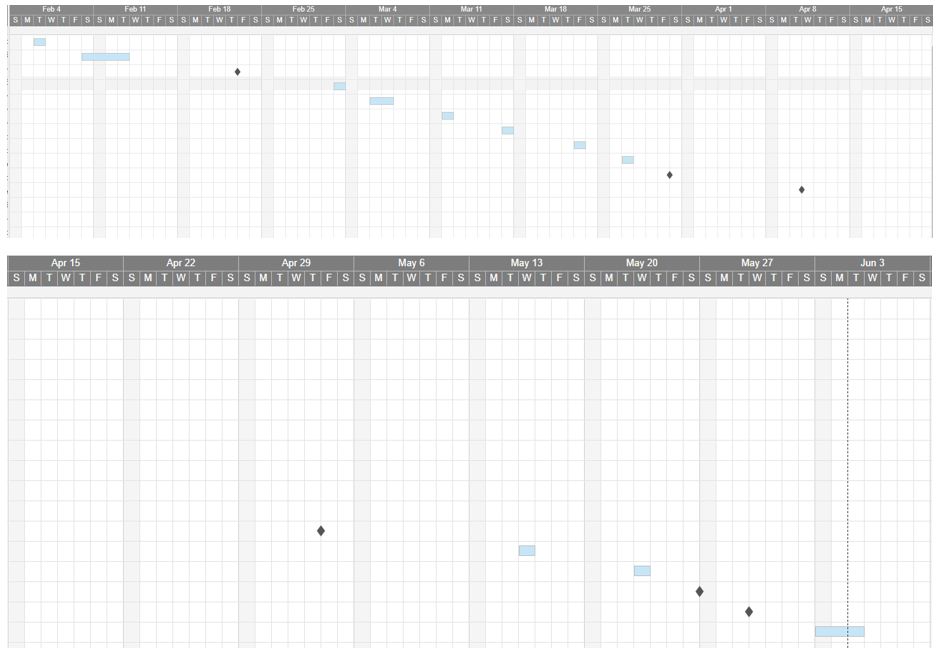
\includegraphics[width=\textwidth]{economy_wt_supervisor}
	\caption{Календарний графік виконання робіт керівника проекту}
	\label{fig:economy_wt_supervisor}
\end{figure} 

\begin{figure}[H]
	\centering
	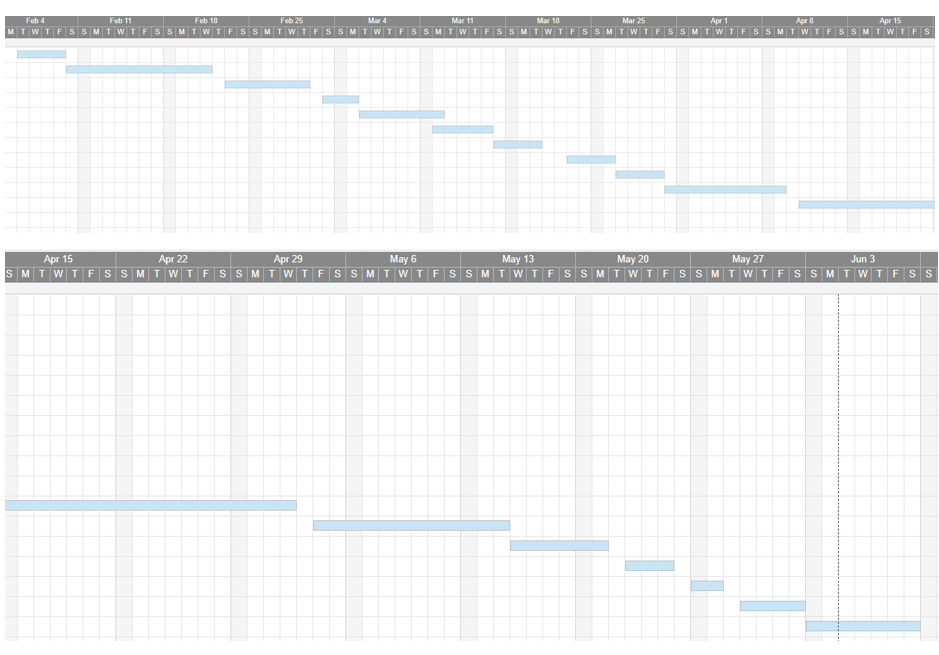
\includegraphics[width=\textwidth]{economy_wt_developer}
	\caption{Календарний графік виконання робіт програміста}
	\label{fig:economy_wt_developer}
\end{figure} 

\subsection{Розрахунок затрат на розробку проекту}
Капітальні вкладення в проекти, пов'язані з розробкою та впровадженням програмних продуктів, розраховуються за формулою
\begin{equation}\label{eq:economy_k}
	K=K_\textup{п} + K_\textup{р},
\end{equation}
\begin{description}
	\item[де] $K_\textup{п}$ --- капітальні вкладення на проектування, грн.;
	\item $K_\textup{р}$ --- капітальні вкладення на реалізацію проекту, грн.
\end{description}

Виробничі витрати являють собою одноразові витрати на розробку забезпечувальних або функціональних систем, або їх елементів на всіх етапах проектування, а також витрати на їх удосконалення.

Сумарні витрати на проектування системи, її розробку і налагодження на комп'ютері визначаються за формулою:
\begin{equation}\label{eq:economy_k_p}
	K_\textup{п} = ((1 + W_d)(1 + W_c) + W_H) \cdot \sum^m_{i=1} C_\textup{о i} + C_\textup{М} + C_\textup{МЧ}, 
\end{equation}
\begin{description}
	\item[де] $m$ --- кількість робітників, які приймають участь у розробці проекту;
	\item $C_\textup{о i}$ --- витрати на основну заробітну плату робітника $i$-ї категорії, грн.;
	\item $W_d$ --- коефіцієнт, що враховує додаткову заробітну плату в частках до основної заробітної плати ($W_d=40\%$);
	\item $W_c$ --- коефіцієнт, що враховує податок з фізичних осіб та військовий збір, в частках до суми основної та додаткової заробітної плати розробників ($W_c=19.5\%$);
	\item $W_H$ --- коефіцієнт, що враховує податок з фізичних осіб та військовий збір, в частках до суми основної та додаткової заробітної плати розробників ($W_H=60\%$);
	\item $C_\textup{М}$ --- витрати на матеріали;
	\item $C_\textup{МЧ}$ --- витрати на використання машинного часу.
\end{description}

Витрати на основну заробітну плату працівника $i$-ї категорії:
\begin{equation}
	C_\textup{о i} = C_\textup{дні} \cdot t_i,
\end{equation}
\begin{description}
	\item[де] $C_\textup{дні}$ --- денна заробітна плата працівника $i$-ї категорії, грн/день;
	\item $t_i$ --- кількість днів, відпрацьованих працівником $i$-ї категорії. 
\end{description}

Витрати часу на розробку системи по кожному виконавцю приймаються виходячи з його завантаження за календарним графіком виконання робіт (див. таблицю~\ref{tab:economy_wt_calendar}). 

Розрахунок основної заробітної плати розробників проекту наведено у таблиці~\ref{tab:economy_salary} з розрахунку, що в місяці в середньому 22 робочих днів.

{
	\small
	\tabulinesep=1.2mm
	\begin{longtabu} to \textwidth {|X[1,l]|X[1,c]|X[2,c]|X[2,c]|X[1,c]|}
  		\caption{Основна заробітна плата розробників проекту}
  		\label{tab:economy_salary} \\
		\hline
		Посада & Посадовий оклад, грн. & Середня денна ставка, грн. & Витрати часу на розробку, людино-днів & ОЗП, грн. \\
		\hline
		\endfirsthead
  		\caption*{Закінчення таблиці \thetable{}}\\
		\hline
		Посада & Посадовий оклад, грн. & Середня денна ставка, грн. & Витрати часу на розробку, людино-днів & ОЗП, грн. \\
		\hline
		\endhead

		Керівник & 6900 & 313.6 & 16 & 5017.6 \\
		\hline
		Програміст & 1330 & 60.45 & 115 & 6952 \\
		\hline
		\multicolumn{4}{|l|}{Усього} & 11969.9 \\
		\hline

	\end{longtabu}
}

З огляду на те, що проектована інформаційна система повинна бути запрограмована і налагоджена за допомогою комп'ютерів, до сумарних витрат на розробку додаються витрати на використання машинного часу, що обчислюються як
\begin{equation}
	C_\textup{МЧ} = t_\textup{МЧ} \cdot S_\textup{МЧ} \cdot K_\textup{М}
\end{equation}
\begin{description}
	\item[де] $t_\textup{МЧ}$ --- машинний час комп'ютера, необхідний для розробки програмного продукту, $t_\textup{МВ} = 460$ год. (з календарного графіку розробки);
	\item $S_\textup{МЧ}$ --- вартість 1 години машинного часу, $S_\textup{МЧ} = 6$ грн/год;
	\item $K_\textup{М}$ --- коефіцієнт мультипрограмності, $K_\textup{М} = 1$.
\end{description}

{
	\small
	\tabulinesep=1.2mm
	\begin{longtabu} to \textwidth {|X[2,l]|X[1,c]|X[1,c]|X[1,c]|}
  		\caption{Витрати на матеріали}
  		\label{tab:economy_exp_materials} \\
		\hline
		Матеріали & Необхідна кількість & Ціна за одиницю, грн. & Сума, грн. \\
		\hline
		\endfirsthead
  		\caption*{Закінчення таблиці \thetable{}}\\
		\hline
		Матеріали & Необхідна кількість & Ціна за одиницю, грн. & Сума, грн. \\
		\hline
		\endhead

		Зошит загальний & 2 & 10 & 20 \\
		\hline
		Флеш пам'ять USB на 16GB & 1 & 200 & 200 \\
		\hline
		Тонер для принтеру & 1 & 120 & 120 \\
		\hline
		Пачка папіру офісного (300 листів) & 1 & 100 & 100 \\
		\hline
		\multicolumn{3}{|l|}{Усього} & 440 \\
		\hline
	\end{longtabu}
}

Отже, капітальні вкладення на проектування дорівнюють~\eqref{eq:economy_k_p}: 
\begin{align*}
	K_\textup{п} &= (11969.9) \cdot ((1+0.4) \cdot (1+0.195)+0.6)+440+460 \cdot 6 \cdot 1 = \\
	&= 30407.6 \ \textup{грн.}
\end{align*}

{
	\small
	\tabulinesep=1.2mm
	\begin{longtabu} to \textwidth {|X[3,l]|X[1,c]|}
  		\caption{Витрати на розробку}
  		\label{tab:economy_exp_materials} \\
		\hline
		Стаття витрат & Сума, грн. \\
		\hline
		\endfirsthead
  		\caption*{Закінчення таблиці \thetable{}}\\
		\hline
		Стаття витрат & Сума, грн. \\
		\hline
		\endhead

		Основна заробітна плата & 11969.9 \\ \hline
		Додаткова заробітна плата & 4684.3 \\ \hline
		Відрахування на соціальні потреби & 2283.6 \\ \hline
		Витрати на матеріали & 440.0 \\ \hline
		Витрати на машинний час & 2760.0 \\ \hline
		Накладні витрати організації & 7026.0 \\ \hline
		Усього & 30407.6 \\ \hline
	\end{longtabu}
}

У зв'язку з тим, що для впровадження системи, що розглядається в даному проекті, не було витрат, пов'язаних з прокладанням лінії зв'язку, витрат на основне і допоміжне обладнання, витрат на реконструкцію і будівництво будівель, то дані витрати для впровадження системи не враховуються.

Також не приймаються в розрахунок витрати з підготовки та перепідготовки кадрів, витрати на створення інформаційної бази і витрати на придбання типових розробок.

Таким чином, при впровадженні системи, що розглядається в даному проекті, витрати на реалізацію визначаються витратами на обладнання і матеріали. 
У обладнання та матеріали входить комп'ютер, вартість якого 13000 грн.

Тоді витрати на основне і допоміжне обладнання складають
\begin{equation}
	K_o = \sum^n_{j=1} C_{\textup{б}\ j} Q_j Y_j
\end{equation}
\begin{description}
	\item[де] $C_{\textup{б}\ j}$ --- балансова вартість $j$-го виду обладнання, грн., $C_{\textup{б}\ j} = 13000$ грн. при $n = 1$;
	\item $Q_j$ --- кількість одиниць $j$-го обладнання, шт., $Q_j = 1$;
	\item $Y_j$ --- коефіцієнт завантаження $j$-го виду обладнання при обробці інформації за рішенням завдань предметної області.
\end{description}

\begin{equation}
	Y_j = \cfrac{T_j}{\textup{Ф}_{\textup{еф}\ j}}
\end{equation}
\begin{description}
	\item[де] $\textup{Ф}_{\textup{еф}\ j}$ --- ефективний річний фонд часу роботи технічного засобу j-го виду, год./рік.
\end{description}

Час роботи технічного засобу $j$-го виду за рішенням $s$ завдань, год./рік:
\begin{equation}
	T_j = \sum^s_{k=1} t_{k\ j} \cdot U_k,
\end{equation}
\begin{description}
	\item[де] $t_{k\ j}$ --- трудомісткість одноразової обробки інформації по $k$-й задачі на $j$-му виді технічних засобів, годин машинного часу, $t_{k\ j} = 6$;
	\item $U_k$ --- частота (періодичність) рішення $k$-й завдання, днів/рік, $U_k = 250$ на 2018 рік.
\end{description}

Витрати на реалізацію:
\[
	K_\textup{р} = \cfrac{13000 \cdot 1 \cdot 6 \cdot 250}{250 \cdot 8} = 9750 \ \textup{грн.}  
\]

Таким чином, сумарні витрати на розробку проекту складають~\eqref{eq:economy_k}:
\[
	K = K_\textup{п} + K_\textup{р} = 30407.6 + 9750 = 40157.6\ \textup{грн.}  
\]

Розрахуємо сумарні витрати, пов'язані з впровадженням аналога, з яким порівнюється розроблений програмний продукт. Вони складаються з наступних витрат:
\begin{itemize}
	\item витрати на придбання програмного продукту ($80000$ грн.);
	\item витрати на основне і допоміжне обладнання ($13000$ грн.);
	\item витрати з оплати послуг на установку і супровід продукту (безкоштовно протягом перших 3-х років);
	\item витрати на підготовку користувача (підготовчий курс за рахунок компанії у якої покупається ПЗ).
\end{itemize}
Разом сумарні витрати, пов'язані з впровадженням аналога становлять $93000$ грн.

\subsection{Розрахунок експлуатаційних витрат}
До експлуатаційних витрат відносяться витрати, пов'язані із забезпеченням нормального функціонування проекту. 
Ці витрати називають також поточними витратами. 
Поточні витрати розраховуються за формулою
\begin{equation}
	Exp_\textup{пот} = Exp_\textup{зп} + C_\textup{а} + Exp_\textup{е} + C_\textup{рем} + Exp_\textup{м} + Exp_\textup{н}, 
\end{equation}
\begin{description}
	\item[де] $C_\textup{а}$ --- амортизаційні відрахування від вартості обладнання і пристроїв системи, грн.;
	\item $C_\textup{рем}$ --- витрати на поточний ремонт обладнання та пристроїв системи, грн.;
	\item $Exp_\textup{зп}$ --- витрати на зарплату основну та додаткову з відрахуваннями до соціальних фондів, грн.;
	\item $Exp_\textup{е}$ --- витрати на електроенергію, грн.;
	\item $Exp_\textup{м}$ --- витрати на матеріали і носії інформації, грн.;
	\item $Exp_\textup{н}$ --- накладні витрати інформаційного відділу, грн.
\end{description}

Експлуатацію розробленої системи здійснюють фахівці. 
Витрати на їх заробітну плату основну і додаткову з відрахуваннями на соціальні потреби розраховують так:
\begin{equation}
	Exp_\textup{зп} = \sum^m_{i=1} t_i Exp_i (1+W_d)(1 + W_c)
\end{equation}
\begin{description}
	\item[де] $t_i$ --- час експлуатації системи $і$-м працівником, дні;
	\item $Exp_i$ --- середньоденна заробітна плата $і$-го працівника, грн./день.
\end{description}

Дані розрахунку заробітної плати фахівців наведені в таблицях~\eqref{tab:economy_salary_project} і~\eqref{tab:economy_salary_analogue}.

{
	\small
	\tabulinesep=1.2mm
	\begin{longtabu} to \textwidth {|X[2,l]|X[2,c]|X[2,c]|X[2,c]|X[1,c]|}
  		\caption{Дані по заробітній платі фахівців (для проекту)}
  		\label{tab:economy_salary_project} \\
		\hline
		Посада & Посадовий оклад, грн. & Середня денна ставка & Витрати часу на експлуатацію, людино-днів & Фонд з/п, грн. \\
		\hline
		\endfirsthead
  		\caption*{Закінчення таблиці \thetable{}}\\
		\hline
		Посада & Посадовий оклад, грн. & Середня денна ставка & Витрати часу на експлуатацію, людино-днів & Фонд з/п, грн. \\
		\hline
		\endhead

		Співробітник відділу & 4600 & 209.09 & 45 & 15741.3 \\
		\hline
		Програміст & 8900 & 404.6 & 30 & 20306.87 \\
		\hline
		\multicolumn{4}{|l|}{Усього} & 36048.21 \\
		\hline
	\end{longtabu}
}
\[
	C_\textup{зп 1} = (45 \cdot 209.09+30 \cdot 404.6) \cdot 1.4 \cdot 1.195 = 36048.21 \ \textup{грн. (за рік).} 
\]

{
	\small
	\tabulinesep=1.2mm
	\begin{longtabu} to \textwidth {|X[2,l]|X[2,c]|X[2,c]|X[2,c]|X[1,c]|}
  		\caption{Дані по заробітній платі фахівців (для аналогу)}
  		\label{tab:economy_salary_analogue} \\
		\hline
		Посада & Посадовий оклад, грн. & Середня денна ставка & Витрати часу на експлуатацію, людино-днів & Фонд з/п, грн. \\
		\hline
		\endfirsthead
  		\caption*{Закінчення таблиці \thetable{}}\\
		\hline
		Посада & Посадовий оклад, грн. & Середня денна ставка & Витрати часу на експлуатацію, людино-днів & Фонд з/п, грн. \\
		\hline
		\endhead

		Співробітник відділу & 6400 & 290.9 & 60 & 29200.542 \\
		\hline
		Програміст & 11900 & 540.09 & 40 & 36142.82 \\
		\hline
		\multicolumn{4}{|l|}{Усього} & 65343.36 \\
		\hline
	\end{longtabu}
}
\[
	C_\textup{зп 2} = (60 \cdot 290.9 + 40 \cdot 540.09) \cdot 1.4 \cdot 1.195 = 65343.36 \ \textup{грн. (за рік).} 
\]

Сума амортизаційних відрахувань розраховується наступним чином:
\begin{equation}
	C_a = \sum^n_{j=1} \cfrac{C_{\textup{б}\ j} a_j g_j t_j}{F_{\textup{еф}\ j}}
\end{equation}
\begin{description}
	\item[де] $C_{\textup{б}\ j}$ --- балансова вартість $j$-го виду обладнання, грн.;
	\item $a_j$ --- норма річних амортизаційних відрахувань для $j$-го виду обладнання;
	\item $g_j$ --- кількість одиниць обладнання $j$-го виду;
	\item $t_j$ --- час роботи $j$-го виду обладнання, годин;
	\item $F_{\textup{еф}\ j}$ --- ефективний фонд часу роботи обладнання в рік, годин.
\end{description}

Ефективний фонд часу роботи обладнання можна обчислити за формулою:
\begin{equation}
	F_\textup{еф} = D_p \cdot H_e,
\end{equation}
\begin{description}
	\item[де] $D_p$ --- кількість робочих днів в році, $D_p = 250$;
	\item $H_e$ --- норматив середньодобової навантаження, год./день, $H_e= 8$.
\end{description}

Таким чином, ефективний фонд часу роботи обладнання складає $F_\textup{еф} = 250 \cdot 8 = 2000$ годин.

Дані для розрахунку:
\begin{gather*}
	a_j = 0.25, g_j = 1, \\
	t_{j \ \textup{для проекту}} = (45+30) \cdot 8 = 600 \ \textup{год.}, \\
	t_{j \ \textup{для аналогу}} = (60+40) \cdot 8 = 800 \ \textup{год.}, \\
	C_{b1} = 13000 \ \textup{грн.}, C_{b2} = 13000 \ \textup{грн.}
\end{gather*}

Сума амортизаційних відрахувань для проекту складає:
\[
	C_{a\ 1}=\cfrac{13000 \cdot 0.25 \cdot 1 \cdot 600}{2000} = 975 \ \textup{грн.}
\]

Сума амортизаційних відрахувань для аналогу складає: 
\[
	C_{a\ 2}=\cfrac{13000 \cdot 0.25 \cdot 1 \cdot 800}{2000} = 1300 \ \textup{грн.}
\]

Витрати на силову енергію розраховуються за формулою:
\begin{equation}
	Exp_\textup{е} = \sum^n_{j=1} N_j t_j g_j T_\textup{е}
\end{equation}
\begin{description}
	\item[де] $N_j$ --- встановлена потужність $j$-го виду технічних засобів, кВт;
	\item $t_j$ --- час роботи $j$-го виду технічних засобів, годин;
	\item $g_j$ --- коефіцієнт використання встановленої потужності обладнання;
	\item $T_\textup{е}$ --- тариф на електроенергію, грн/кВт год.
\end{description}

В даний час тариф на електроенергію складає 1.68 грн./кВт год, встановлена потужність для комп'ютера дорівнює 0.2 кВт, таким чином витрати на силову енергію для проекту складуть:
\[
Exp_\textup{е} = 0.2 \cdot 1 \cdot 600 \cdot 1.68 = 201.6 \ \textup{грн.}
\]

Для аналогу:
\[
Exp_\textup{е} = 0.2 \cdot 1 \cdot 800 \cdot 1.68 = 268.8 \ \textup{грн.}
\]

Витрати на поточний ремонт обладнання розраховуються за формулою:
\begin{equation}
	C_\textup{рем} = \sum^n_{j=1} \cfrac{C_{p\ j} C_{\textup{б}\ j} T_{p\ j}}{T^i_\textup{еф}},
\end{equation}
\begin{description}
	\item[де] $C_{p\ j}$ --- норматив витрат на ремонт, $C_{p\ j} = 0.05$.
\end{description}

Витрати на поточний ремонт обладнання для проекту складають:
\[
C_\textup{рем 1} = \cfrac{0.05 \cdot 13000 \cdot 600}{2000} = 195 \ \textup{грн.}
\]

Для аналогу:
\[
C_\textup{рем 2} = \cfrac{0.05 \cdot 13000 \cdot 800}{2000} = 260 \ \textup{грн.} 
\]

Витрати на матеріали, які споживаються протягом року, складають 1\% від балансової вартості основного устаткування і рівні $130$ грн. для проекту і аналога.

Накладні витрати включають витрати на утримання адміністративного та управлінського персоналу, на утримання приміщення і т.д. 
Норматив накладних витрат становить 20\% від прямих витрат, що включають перші п'ять статей витрат, представлених в таблиці~\ref{tab:economy_exp_year}.

Накладні витрати для проекту:
\[
C_\textup{н 1} = 0.2 \cdot (36048.21 + 975 + 201.6 + 195 + 220) = 7527.962 \ \textup{грн.} 
\]

Накладні витрати для аналогу:
\[
C_\textup{н 2} = 0.2 \cdot (65343.36 + 1300 + 268.8 + 260 + 220) = 15117.472 \ \textup{грн.} 
\]

{
	\small
	\tabulinesep=1.2mm
	\begin{longtabu} to \textwidth {|X[3,l]|X[1,c]|X[1,c]|}
  		\caption{Річні експлуатаційні витрати}
  		\label{tab:economy_exp_year} \\
		\hline
		Стаття витрат & Витрати на проект, грн. & Витрати на аналог, грн. \\
		\hline
		\endfirsthead
  		\caption*{Закінчення таблиці \thetable{}}\\
		\hline
		Стаття витрат & Витрати на проект, грн. & Витрати на аналог, грн. \\
		\hline
		\endhead

		Основна і додаткова зарплата з відрахуваннями & 36048.21 & 65343.36 \\
		\hline
		Амортизаційні відрахування & 975 & 1300 \\
		\hline
		Витрати на електроенергію & 201.6 & 268.8 \\
		\hline
		Витрати на поточний ремонт & 195 & 260 \\
		\hline
		Витрати на матеріали & 130 & 130 \\
		\hline
		Накладні витрати & 7527.962 & 15117.472 \\
		\hline
		Усього & 45077.772 & 82419.632 \\
		\hline
	\end{longtabu}
}

\subsection{Оцінка ефективності розробленого проекту}
Оцінка економічної ефективності варіантів проектних рішень елементів АІС ґрунтується на розрахунку показників порівняльної економічної ефективності капітальних вкладень.
Річний економічний ефект від використання розроблюваної системи визначається по різниці приведених витрат на базовий і новий варіанти в розрахунку на річний обсяг виконуваних робіт:
\begin{equation}
	E = N \cdot (Exp_1 \cdot A_\textup{к} - Exp_2)
\end{equation}
\begin{description}
	\item[де] $Exp_1$, $Exp_2$ --- наведені витрати на одиницю робіт, що виконуються за допомогою базового і проектованого варіантів процесу обробки інформації, грн.;
	\item $N$ --- обсяг робіт, виконуваних за допомогою розробленого продукту, $N = 1$.
\end{description}

Наведені витрати на одиницю робіт, виконуваних за базовим і розробляється варіантів, розраховуються за формулою:
\begin{equation}
	Exp_j = C_j + E_\textup{н} \cdot K_j
\end{equation}
\begin{description}
	\item[де] $C_j$ --- поточні експлуатаційні витрати одиниці робіт, грн.;
	\item $E_\textup{н}$ --- нормативний коефіцієнт економічної ефективності, $E_\textup{н} = 0.33$;
	\item $K_j$ --- сумарні витрати, пов'язані з впровадженням нового проекту.
\end{description}

Витрати на одиницю робіт по проекту:
\[
	Exp_1= 45077.772+0.33 \cdot 40157.6  = 58329.78 \ \textup{грн.}
\]

Витрати на одиницю робіт по аналогу:
\[
	Exp_2= 82419.632+0.33 \cdot 93000  = 113109.632 \ \textup{грн.}
\]

Економічний ефект від використання розроблюваної системи:
\[
	E = 113109.632 \cdot 1.1722 - 58329.78  = 74257.3306 \ \textup{грн.}
\]

Зведені дані по розрахунку економічного ефекту наведені в таблиці~\eqref{tab:economy_effect}.

{
	\small
	\tabulinesep=1.2mm
	\begin{longtabu} to \textwidth {|X[3,l]|X[1,c]|X[1,c]|}
  		\caption{Економічний ефект}
  		\label{tab:economy_effect} \\
		\hline
		\multirow{2}{*}{Характеристика} & \multicolumn{2}{|c|}{Значення}  \\
		\cline{2-3}
		& Продукт-аналог (базовий) & Розроблюваний програмний продукт \\
		\hline
		\endfirsthead
  		\caption*{Закінчення таблиці \thetable{}}\\
		\hline
		\multirow{2}{*}{Характеристика} & \multicolumn{2}{|c|}{Значення}  \\
		\cline{2-3}
		& Продукт-аналог (базовий) & Розроблюваний програмний продукт \\
		\hline
		\endhead

		Собівартість (поточні експлуатаційні витрати), грн. & 82419.632 & 45077.772 \\
		\hline
		Сумарні витрати, пов'язані з впровадженням проекту, грн. & 93000 & 40157.6 \\
		\hline
		Наведені витрати на одиницю робіт, грн. & 113109.632 & 58329.78 \\
		\hline
		Економічний ефект від використання розроблюваної системи (програмного продукту), грн. & \multicolumn{2}{|c|}{74257.3306} \\
		\hline
	\end{longtabu}
}

Після визначення річного економічного ефекту необхідно розрахувати термін окупності витрат на розробку продукту за формулою:
\begin{equation}
	T_\textup{ок} = \cfrac{K}{E}. 
\end{equation}

Термін окупності складе:
\[
	T_\textup{ок} = \cfrac{113109.632}{74257.3306} = 1.52 \ \textup{року (19 місяців).}
\]

Потім розрахуємо фактичний коефіцієнт економічної ефективності розробки $E_\textup{ф}$ і порівняємо його з нормативним значенням коефіцієнта ефективності капітальних вкладень $E_\textup{н} = 0.33$:
\[
	E_\textup{ф} = \cfrac{1}{T_\textup{ок}} = \cfrac{1}{1.52} = 0.6565.
\]

Фактичний коефіцієнт економічної ефективності розробки вийшов більше, ніж нормативний ($0.6565 > 0.33$), тому розробка та впровадження розроблюваного продукту є ефективною.

Таким чином, в ході проробленої роботи знайдені всі необхідні дані, що доводять доцільність і ефективність розроблюваної системи.

